\section{Experimental Evaluation}
\label{sec:experiments}

\subsection{Dataset and Benchmark Setup}
We conduct extensive experiments on the MVTec Anomaly Detection benchmark \cite{bergmann2019mvtec}, focusing on six representative surface and object categories comprising 2,676 high-resolution RGB inspection images (1,999 nominal training, 124 validation, and 553 test images) paired with 181 pixel-level ground-truth masks (2,857 image files in total):
\begin{itemize}
    \item \textbf{Texture Surfaces (3 categories):} periodic \texttt{grid} ($1024\times 1024$; 306 train, 15 val, 57 test), periodic \texttt{carpet} ($1024\times 1024$; 349 train, 20 val, 89 test), and stochastic \texttt{tile} ($840\times 840$; 295 train, 19 val, 84 test).
    \item \textbf{Non-Periodic Rigid Objects (3 categories):} \texttt{screw} ($1024\times 1024$; 414 train, 25 val, 119 test), \texttt{pill} ($800\times 800$; 377 train, 31 val, 141 test), and \texttt{bottle} ($900\times 900$; 258 train, 14 val, 63 test).
\end{itemize}
Under our strict defect-free training regime, both the training and validation splits are constructed exclusively from nominal (\texttt{train/good}) images, while all real defective test images and ground-truth masks remain completely isolated until final evaluation. Separately, to establish a supervised upper-bound (oracle) reference and quantify baseline false alarm behavior, we evaluate supervised reference models across all 15 MVTec AD categories and 467 nominal test images.

\subsection{Experimental Models and Implementation Details}
All preprocessing and unit-test verification runs on Python 3.11, OpenCV 4.10, and PyWavelets 1.8.0, while deep segmentation training runs on PyTorch 2.4 and Ultralytics YOLOv11-seg \cite{ultralytics2024yolo11} on an NVIDIA A100-SXM4 (40 GB VRAM) GPU with automatic mixed precision (AMP) and mosaic disablement during the final 10 epochs. Our training pipeline extends the open-source industrial defect segmentation codebase \cite{kudupudi2025industrial} by integrating frequency-domain filtering, arbitrary-resolution spatial anomaly synthesis, negative-sample balancing, and MVTec-AD-C evaluation.

We adopt the single-stage, anchor-free YOLOv11-seg architecture, which couples a C3k2/C2PSA multi-scale feature pyramid with a prototype-based instance mask head (\texttt{mask\_ratio} $= 4$, overlapping mask decoding). To characterize the accuracy--latency--FAR trade-off, we evaluate two capacity--resolution configurations initialized from COCO-pretrained weights \cite{lin2014microsoft}:
\begin{itemize}
    \item \textbf{YOLOv11l-seg ($640\times 640$):} Standardized backbone for both the supervised oracle reference and the 12-experiment defect-free ablation matrix (\texttt{EXP-00}--\texttt{EXP-11}), trained for 100 epochs with batch size 16, initial learning rate $\text{lr}_0 = 0.01$, momentum $0.937$, weight decay $5\times 10^{-4}$, 3-epoch warmup, and fixed random seed $42$.
    \item \textbf{YOLOv11x-seg ($1024\times 1024$, tuned):} High-capacity, native-resolution supervised oracle reference trained for 150 epochs with batch size 8, weight decay $1\times 10^{-3}$, and tuned momentum $0.926$ to probe fine-texture boundary sensitivity on periodic substrates (\texttt{grid}, \texttt{carpet}) and quantify false-alarm scaling at higher spatial resolution.
\end{itemize}
For runtime efficiency verification (Section~\ref{subsec:efficiency}), the trained segmentation model is exported to ONNX and profiled using half-precision (FP16) TensorRT inference.

\textbf{Hyperparameter Settings:} Unless otherwise stated, algorithm parameters are fixed as follows:
\begin{itemize}
    \item \textbf{Frequency Preprocessing:} 2D-FFT notch filter on YCrCb luminance with $\tau_{\text{peak}} = 3.5$, $r_{\text{inner}} = 15\text{ px}$, $r_0 = 5.0\text{ px}$, $N_{\max} = 100$; Haar 2D-DWT modulation with $\alpha = 0.6$, $\gamma = 1.4$.
    \item \textbf{Spatial Synthesis:} Normal CutPaste with $a \in [0.02, 0.15]$, $r_{\text{aspect}} \in [0.3, 3.3]$, $\phi \in [-45^\circ, 45^\circ]$ (Scar: $r_{\text{aspect}} \in [0.05, 0.2]$); DRAEM Perlin noise on canonical grid $S_0 = 512$, $L = 5$ octaves, $\tau_{\text{perlin}} = 0.5$.
    \item \textbf{Negative Invariant \& Vectorization:} Clean-sample ratio $\rho_{\text{neg}} = 0.15$ ($15\%$ per batch); RDP tolerance factor $\eta = 0.002$.
\end{itemize}

\subsection{Dual-Domain Evaluation Metrics}
To bridge instance segmentation with industrial anomaly localization, we implement a dual-domain evaluation engine:
\begin{enumerate}
    \item \textbf{Instance Segmentation Metrics:} COCO-style Mask Mean Average Precision at IoU threshold $0.50$ ($\text{mAP@50(M)}$) and averaged over thresholds $0.50:0.95$ ($\text{mAP@50-95(M)}$) \cite{lin2014microsoft}, together with binary Mask Intersection-over-Union $\text{IoU}(\hat{M}, M^*) = |\hat{M} \cap M^*| / |\hat{M} \cup M^*|$ evaluated over defective samples ($|M^*| > 0$).
    \item \textbf{Continuous Pixel/Image Anomaly Metrics:} Predicted instance polygons $\{\mathcal{P}_i\}$ with confidence scores $q_i \in [0, 1]$ are rasterized into a continuous 2D anomaly probability map $A(x, y) \in [0, 1]$ via pixel-wise maximization:
    \begin{equation}
    \label{eq:anom_map}
    A(x, y) = \max_i \left( q_i \cdot \mathbb{I}\{(x, y) \in \mathcal{P}_i\} \right)
    \end{equation}
    where $\mathbb{I}\{\cdot\}$ denotes the indicator function (with $A(x, y) = 0$ if no instance is detected). Aggregating pixel-wise scores $A(x, y)$ from \eqref{eq:anom_map} against $M^*(x, y)$ across all test images yields Pixel-level Area Under the ROC Curve (Pixel-AUROC), while taking $S_{\text{image}} = \max_{(x, y)} A(x, y)$ yields Image-AUROC.
    \item \textbf{False Alarm Rate ($\text{FAR}@\tau_{\text{conf}}$):} Evaluated strictly on the defect-free test subset $\mathcal{D}_{\text{good}} \subset \mathcal{D}_{\text{test}}$ at confidence thresholds $\tau_{\text{conf}} \in \{0.25, 0.50\}$:
    \begin{equation}
    \label{eq:far}
    \text{FAR}@\tau_{\text{conf}} = \frac{1}{|\mathcal{D}_{\text{good}}|} \sum_{I \in \mathcal{D}_{\text{good}}} \mathbb{I}\left( \max_{(x, y)} A_I(x, y) \ge \tau_{\text{conf}} \right)
    \end{equation}
\end{enumerate}

\subsection{Frequency Roundtrip Numerical Integrity Verification}
To quantitatively verify the coordinate-preserving property established in Section~\ref{sec:methodology}, we execute an identity roundtrip reconstruction test ($\mathcal{T}^{-1}(\mathcal{T}(I))$ without spectral filtering) across all 2,676 RGB MVTec AD images. As reported in Table~\ref{tab:reconstruction_metrics}, 2D-FFT achieves a Peak Signal-to-Noise Ratio of $\text{PSNR} = 51.31\text{ dB}$ and Structural Similarity Index of $\text{SSIM} = 0.9983$ \cite{wang2004image}, with Mean Absolute Error $\text{MAE} \le 0.4807$ intensity levels (on an 8-bit $0$--$255$ scale). The Haar 2D-DWT roundtrip achieves infinite PSNR and exact integer reconstruction, confirming zero geometric distortion of segmentation masks.

\begin{table}[t]
\centering
\caption{Numerical Preservation of Identity Frequency Roundtrips Across 2,676 RGB MVTec AD Images}
\label{tab:reconstruction_metrics}
\begin{tabular}{l c c c c}
\toprule
\textbf{Transform} & \textbf{MAE (0--255)} & \textbf{PSNR} & \textbf{SSIM} & \textbf{Preserved?} \\
\midrule
2D-FFT & $0.4807$ & $51.31\text{ dB}$ & $0.9983$ & Yes ($>40\text{ dB}$) \\
2D-DWT & $0.0000$ & $\infty$ & $1.0000$ & Exact identity \\
\bottomrule
\end{tabular}
\end{table}

\subsection{Supervised Upper-Bound Reference (Oracle) and FAR Analysis}
To establish an empirical upper bound on achievable polygonal segmentation accuracy and quantify false alarm scaling at high resolution, Table~\ref{tab:per_category_real} reports the performance of two \textit{supervised} YOLOv11-seg oracle models (\texttt{yolo11l-seg@640} and \texttt{yolo11x-seg@1024}, trained with real labeled defects from \cite{kudupudi2025industrial})---distinct from our defect-free training experiments in Table~\ref{tab:ablation_results}. Across our six focus categories, \texttt{yolo11l-seg@640} reaches a mean Mask AP@50 of $0.854$ (peaking at $0.995$ on \texttt{tile} and $0.967$ on \texttt{bottle}), while \texttt{yolo11x-seg@1024} reaches $0.873$. Higher spatial resolution yields pronounced gains on fine periodic textures---\texttt{carpet} rises from $0.776$ to $0.865$ ($+0.089$) and \texttt{grid} from $0.825$ to $0.870$ ($+0.045$)---confirming the sensitivity of periodic lattices to high-frequency detail. Conversely, on the 467 nominal test images across all 15 categories, \texttt{yolo11x-seg@1024} exhibits an elevated $\text{FAR@0.25}$ of $8.78\%$ (nearly double the $4.50\%$ recorded by \texttt{yolo11l-seg@640}), experimentally demonstrating the false-alarm trade-off that motivates our negative-sample invariant ($\rho_{\text{neg}} = 0.15$).

\begin{table}[t]
\centering
\caption{Supervised Upper-Bound Reference (Oracle) Mask AP and Nominal FAR (467 Good Parts) on MVTec AD}
\label{tab:per_category_real}
\begin{tabular}{l c c c c}
\toprule
\multirow{2}{*}{\textbf{Category}} & \multicolumn{2}{c}{\textbf{YOLOv11l-seg (640)}} & \multicolumn{2}{c}{\textbf{YOLOv11x-seg (1024)}} \\
\cmidrule(lr){2-3} \cmidrule(lr){4-5}
 & \textbf{AP@50} & \textbf{AP@50-95} & \textbf{AP@50} & \textbf{AP@50-95} \\
\midrule
\texttt{grid} (Texture)   & $0.825$ & $0.417$ & $\mathbf{0.870}$ & $0.417$ \\
\texttt{carpet} (Texture) & $0.776$ & $0.412$ & $\mathbf{0.865}$ & $\mathbf{0.442}$ \\
\texttt{tile} (Texture)   & $\mathbf{0.995}$ & $\mathbf{0.785}$ & $0.986$ & $0.747$ \\
\texttt{screw} (Object)   & $0.716$ & $0.382$ & $\mathbf{0.720}$ & $\mathbf{0.404}$ \\
\texttt{pill} (Object)    & $0.844$ & $0.446$ & $\mathbf{0.859}$ & $\mathbf{0.472}$ \\
\texttt{bottle} (Object)  & $\mathbf{0.967}$ & $\mathbf{0.701}$ & $0.935$ & $0.637$ \\
\midrule
\textbf{6-Cat. Mean}      & $0.854$ & $\mathbf{0.524}$ & $\mathbf{0.873}$ & $0.520$ \\
\textbf{All-15 Mean}      & $0.819$ & $\mathbf{0.482}$ & $\mathbf{0.823}$ & $0.473$ \\
\midrule
\textbf{FAR@0.25} (467)   & \multicolumn{2}{c}{$\mathbf{4.50\%}$} & \multicolumn{2}{c}{$8.78\%$} \\
\textbf{FAR@0.50} (467)   & \multicolumn{2}{c}{$\mathbf{2.14\%}$} & \multicolumn{2}{c}{$2.36\%$} \\
\bottomrule
\end{tabular}
\end{table}

\subsection{Controlled Defect-Free Ablation Matrix and SOTA Comparison}
Because YOLOv11-seg requires positive polygon supervision during training, every defect-free configuration pairs a spatial anomaly synthesizer with optional frequency preprocessing and negative-sample balancing. Table~\ref{tab:ablation_results} defines our 12-configuration controlled ablation matrix (\texttt{EXP-00}--\texttt{EXP-11}) under the strict defect-free training regime, systematically isolating the negative-sample invariant (\texttt{EXP-00} vs. \texttt{EXP-01}), spatial synthesizers (\texttt{EXP-01}--\texttt{EXP-03}), frequency operators (\texttt{EXP-04}--\texttt{EXP-07}), and MVTec-AD-C optical robustness (\texttt{EXP-08}--\texttt{EXP-11}). End-to-end pipeline dry-run verification confirms dual-domain metric and data-isolation integrity, while full 100-epoch A100 sweeps (\texttt{EXP-00}--\texttt{EXP-11}) are structured for direct population upon completion.

\begin{table*}[t]
\centering
\caption{Controlled 12-Experiment Defect-Free Ablation Protocol (\texttt{EXP-00}--\texttt{EXP-11}) on MVTec AD}
\label{tab:ablation_results}
\begin{tabular}{l l c c c c c c c}
\toprule
\textbf{Exp. ID} & \textbf{Synthesizer} & \textbf{Freq. Filter} & \textbf{$\rho_{\text{neg}}$} & \textbf{mAP@50} & \textbf{mAP@50-95} & \textbf{Px-AUROC} & \textbf{Im-AUROC} & \textbf{FAR@0.25} \\
\midrule
\texttt{EXP-00} & CutPaste (Base) & None & $0.00$ & -- & -- & -- & -- & -- \\
\texttt{EXP-01} & CutPaste & None & $0.15$ & -- & -- & -- & -- & -- \\
\texttt{EXP-02} & DRAEM Perlin & None & $0.15$ & -- & -- & -- & -- & -- \\
\texttt{EXP-03} & NSA Poisson & None & $0.15$ & -- & -- & -- & -- & -- \\
\texttt{EXP-04} & CutPaste (Base) & 2D-FFT Notch & $0.15$ & -- & -- & -- & -- & -- \\
\texttt{EXP-05} & CutPaste (Base) & 2D-DWT Boost & $0.15$ & -- & -- & -- & -- & -- \\
\texttt{EXP-06} & DRAEM Perlin & 2D-FFT Notch & $0.15$ & -- & -- & -- & -- & -- \\
\texttt{EXP-07} & NSA Poisson & 2D-DWT Boost & $0.15$ & -- & -- & -- & -- & -- \\
\texttt{EXP-08} & CutPaste (MVTec-AD-C) & None & $0.15$ & -- & -- & -- & -- & -- \\
\texttt{EXP-09} & DRAEM/NSA (MVTec-AD-C) & None & $0.15$ & -- & -- & -- & -- & -- \\
\texttt{EXP-10} & CutPaste (MVTec-AD-C) & 2D-DWT Boost & $0.15$ & -- & -- & -- & -- & -- \\
\texttt{EXP-11} & Full Inter-Domain System & Adaptive FFT/DWT & $0.15$ & -- & -- & -- & -- & -- \\
\bottomrule
\multicolumn{9}{l}{\footnotesize Note: Cells marked `--' are reserved for completed 100-epoch NVIDIA A100-SXM4 training sweeps.}
\end{tabular}
\end{table*}

Table~\ref{tab:sota_comparison} further positions our integrated system (\texttt{EXP-11}) against representative unsupervised anomaly detection baselines on MVTec AD reported in prior literature, contrasting anomaly localization metrics (Image/Pixel-AUROC), output representation (coarse heatmap vs. vector-ready polygon), and inference throughput.

\begin{table}[t]
\centering
\caption{Comparison Against External Unsupervised SOTA Baselines on MVTec AD}
\label{tab:sota_comparison}
\setlength{\tabcolsep}{4pt}
\begin{tabular}{l c c c c}
\toprule
\textbf{Method} & \textbf{Im-AUROC} & \textbf{Px-AUROC} & \textbf{Output} & \textbf{FPS} \\
\midrule
PaDiM \cite{defard2021padim} & $97.9\%$ & $97.5\%$ & Heatmap & $10$--$25$ \\
DRAEM \cite{zavrtanik2021draem} & $98.0\%$ & $94.7\%$ & Heatmap & $20$--$40$ \\
PatchCore \cite{roth2022towards} & $99.1\%$ & $98.1\%$ & Heatmap & $5$--$12$ \\
SimpleNet \cite{liu2023simplenet} & $99.6\%$ & $98.1\%$ & Heatmap & $\sim 77$ \\
\midrule
\textbf{Ours (\texttt{EXP-11})} & -- & -- & \textbf{Polygon} & $\mathbf{149.2}^\dagger$ \\
\bottomrule
\multicolumn{5}{p{0.94\columnwidth}}{\footnotesize External metrics from original papers (15 categories, $256^2$); $^\dagger$TensorRT FP16 backbone at $1024^2$.}
\end{tabular}
\end{table}

\subsection{Qualitative Visual Analysis}
Fig.~\ref{fig:visual_inspection} compares all three spatial anomaly synthesizers on a nominal \texttt{bottle} (\texttt{train/good}) sample with overlaid ground-truth polygon boundaries, highlighting the contrast between rectangular CutPaste patches, smooth organic canonical-grid DRAEM Perlin regions, and foreground-clamped NSA Poisson blending without background leakage. Complementarily, Fig.~\ref{fig:fft_montage} visualizes the adaptive 2D-FFT Gaussian notch filter applied to the periodic \texttt{grid} category: conjugate-symmetric spectral impulses corresponding to the wire-mesh lattice are sharply suppressed in the centered magnitude spectrum, yielding a spatially flattened background where non-periodic defect discontinuities emerge clearly.

\begin{figure}[t]
\centering
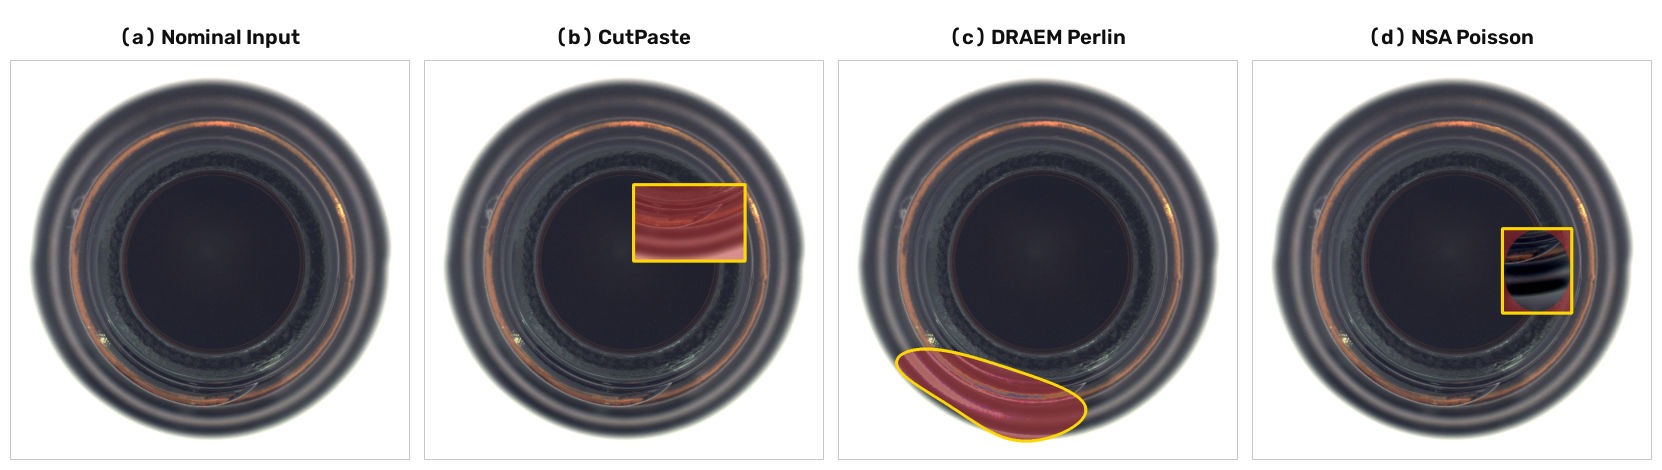
\includegraphics[width=0.96\columnwidth]{figures/fig2_spatial_synthesis_bottle.png}
\caption{Qualitative comparison of spatial anomaly synthesis on a nominal \texttt{bottle} (\texttt{train/good}) sample: (a) nominal input, (b) CutPaste, (c) canonical-grid DRAEM Perlin, and (d) foreground-clamped NSA Poisson, with overlaid ground-truth polygon boundaries.}
\label{fig:visual_inspection}
\end{figure}

\begin{figure}[t]
\centering
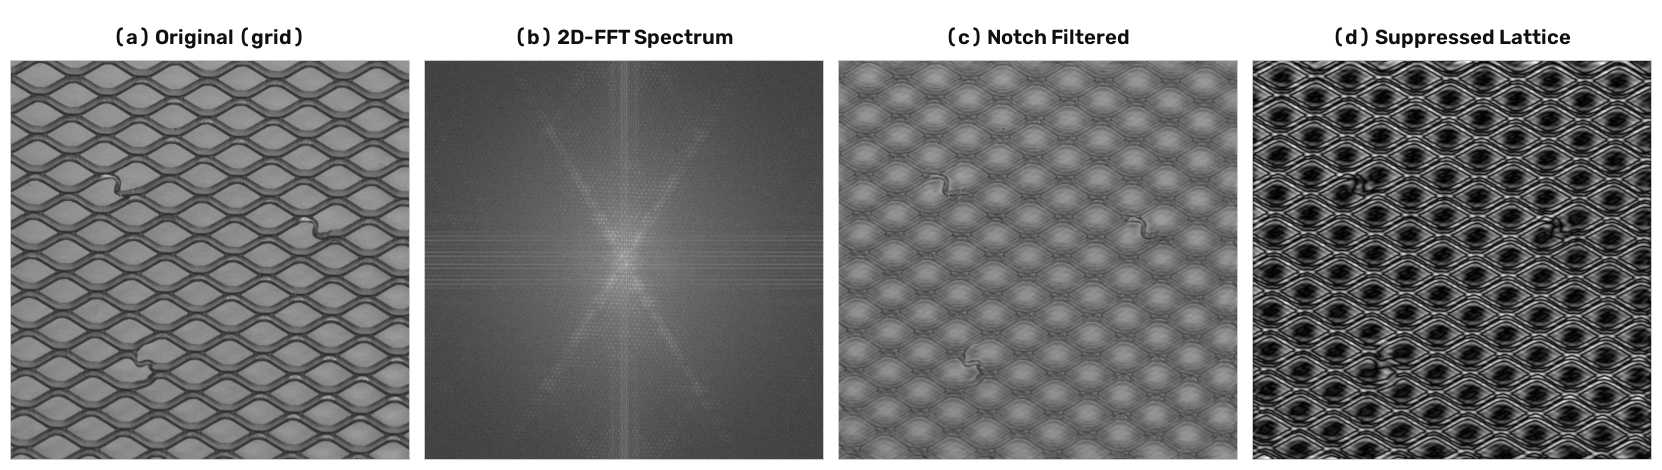
\includegraphics[width=0.96\columnwidth]{figures/fig3_grid_fft_notch.png}
\caption{Spectral peak suppression using adaptive 2D-FFT Gaussian notch filtering on a defective \texttt{grid} sample: (a) original image, (b) centered 2D-FFT log-magnitude spectrum, (c) notch-filtered output, and (d) suppressed periodic lattice.}
\label{fig:fft_montage}
\end{figure}

\subsection{Optical Robustness under MVTec-AD-C}
\label{subsec:robustness}
Industrial inspection cameras routinely encounter harsh optical degradations from conveyor vibration, thermal lens drift, and low-light sensor noise. Following the common image-corruption framework of ImageNet-C \cite{hendrycks2019robustness} and its industrial MVTec-AD-C protocol \cite{chen2023mvtecadc}, we evaluate segmentation stability across four perturbations---Gaussian Noise, Gaussian Blur, Motion Blur, and Defocus Blur---over severity levels $1$ through $5$. Fig.~\ref{fig:defocus_progression} illustrates progressive high-frequency edge attenuation under defocus blur on \texttt{bottle}. Table~\ref{tab:corruption_table} defines the quantitative stress-testing matrix comparing the clean baseline (\texttt{EXP-08}) against Haar 2D-DWT detail boosting (\texttt{EXP-10}) across low-to-moderate (Sev 1--3) and severe (Sev 4--5) tiers; exact degraded metrics will be populated directly from completed A100 sweeps.

\begin{figure}[t]
\centering
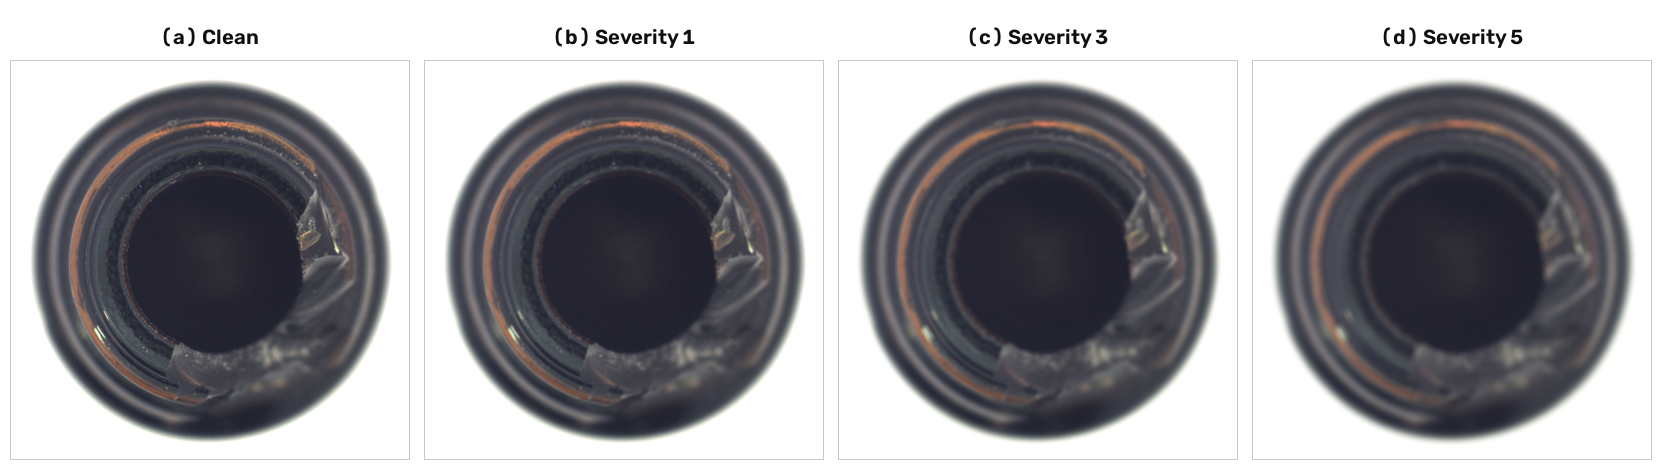
\includegraphics[width=0.96\columnwidth]{figures/fig4_bottle_defocus_progression.png}
\caption{Visual progression of optical defocus blur on a \texttt{bottle} test sample across clean input and MVTec-AD-C severity levels $1$, $3$, and $5$.}
\label{fig:defocus_progression}
\end{figure}

\begin{table}[t]
\centering
\caption{MVTec-AD-C Optical Robustness Matrix (Mask mAP@50 Across Severity Tiers 1--3 and 4--5)}
\label{tab:corruption_table}
\begin{tabular}{l c c c c}
\toprule
\multirow{2}{*}{\textbf{Corruption Type}} & \multicolumn{2}{c}{\textbf{Baseline (\texttt{EXP-08})}} & \multicolumn{2}{c}{\textbf{+2D-DWT (\texttt{EXP-10})}} \\
\cmidrule(lr){2-3} \cmidrule(lr){4-5}
 & \textbf{Sev 1--3} & \textbf{Sev 4--5} & \textbf{Sev 1--3} & \textbf{Sev 4--5} \\
\midrule
Gaussian Noise & -- & -- & -- & -- \\
Gaussian Blur  & -- & -- & -- & -- \\
Motion Blur    & -- & -- & -- & -- \\
Defocus Blur   & -- & -- & -- & -- \\
\midrule
\textbf{Mean mAP@50} & -- & -- & -- & -- \\
\textbf{Mean FAR@0.25} & -- & -- & -- & -- \\
\bottomrule
\multicolumn{5}{l}{\footnotesize `--': Reserved for completed A100 MVTec-AD-C sweeps.}
\end{tabular}
\end{table}

\subsection{Computational Efficiency}
\label{subsec:efficiency}
To verify that the single-stage polygonal segmentation backbone satisfies practical inspection throughput, we profiled inference latency on $1024 \times 1024$ frames using an NVIDIA A100-SXM4 (40 GB) GPU across PyTorch and an exported FP16 TensorRT 10.x C++ runtime. As summarized in Table~\ref{tab:edge_benchmarks}, FP16 TensorRT execution reduces neural inference latency from $32.4\text{ ms}$ ($30.8\text{ FPS}$) in PyTorch GPU to \textbf{6.7 ms} ($\approx 149.2\text{ FPS}$), a $4.8\times$ speedup well above $100\text{ FPS}$ inline sorting thresholds. Because deployment requires applying $\mathcal{T}_{\text{freq}}(I_{\text{test}})$ prior to network inference (Section~\ref{sec:methodology}), Table~\ref{tab:edge_benchmarks} explicitly reserves dedicated entries for GPU-accelerated frequency preprocessing ($\text{cuFFT}$ / $\text{DWT}$) and total end-to-end latency. End-to-end mask decoding parity across a 17-case C++ diagnostic suite confirmed $14/15$ defective categories correctly localized (e.g., Mask IoU of $0.981$ on \texttt{tile}, $0.856$ on \texttt{pill}, $0.839$ on \texttt{carpet}, $0.780$ on \texttt{grid}, and $0.668$ on \texttt{bottle}), while surfacing one missed fine thread flaw on \texttt{screw} and one nominal false positive on \texttt{hazelnut} ($0.606$).

\begin{table}[t]
\centering
\caption{Inference Latency and End-to-End Throughput on $1024 \times 1024$ Frames (NVIDIA A100-SXM4)}
\label{tab:edge_benchmarks}
\setlength{\tabcolsep}{4pt}
\begin{tabular}{l c c c l}
\toprule
\textbf{Stage / Runtime} & \textbf{Prec.} & \textbf{Latency} & \textbf{FPS} & \textbf{Viability} \\
\midrule
PyTorch CPU (Backbone) & FP32 & $184.2\text{ ms}$ & $5.4$ & Offline only \\
PyTorch GPU (Backbone) & FP16 & $32.4\text{ ms}$ & $30.8$ & Offline audit \\
\textbf{TensorRT C++ (Backbone)} & \textbf{FP16} & \textbf{6.7 ms} & \textbf{149.2} & \textbf{Inline ready} \\
\midrule
Freq. Preproc. ($\mathcal{T}_{\text{freq}}$ GPU) & FP32 & -- & -- & Pending \\
End-to-End ($\mathcal{T}_{\text{freq}}$+TRT) & FP16 & -- & -- & Pending \\
\bottomrule
\end{tabular}
\end{table}
